\chapter{モデルベースシステムズエンジニアリング}
%高井さん
\label{chap4}

\section{システムエンジニアリングの基礎}

\subsection{システムエンジニアリングとは}

システムエンジニアリングは、INCOSE SE HANDBOOKによると、「システムの実現を成功させることができる複数の専門分野にまたがるアプローチおよび手段」と定義されています。この分野は以下の役割を果たします:

\begin{itemize}
    \item システム開発に必要な概念の提供
    \item システム開発で必要な活動の提供
\end{itemize}

システムエンジニアリングは、分野に依存せず「システム」を構築したり発展させたりするための知見をまとめたものです。従来は、製品やサービスの領域毎に、開発プロセスは発展し、その中での最適化が行われてきました。しかし、多くのシステムが大規模化、複雑化するなかで、領域毎に発展してきた方法論では、必要な納期を満たせなかったり品質を保証することが難しくなってきました。一方で、そのような課題は、製品やサービスに依存しない現象として説明したり、さらにはその解決アプローチについても、一般化して検討できるかもしれない、と気付いた人たちがいました。そのような知見をまとめたものがシステムズエンジニアリングであり、実際多くの現場でその効果が確かめられたため、国際標準化なども含めて普及が進んでいます。

前述の通り、システムが大規模化、複雑化すると、複数の製品やサービス領域を組み合わせることが一般的になり、これまで交流のなかった技術者も共同作業をしなければなりません。そのようなときに共通言語を与えるのも、システムズエンジニアリングの役割です。また、大規模かつ複雑なシステムは、その開発や運用プロセスも複雑になり、その計画を立てたり、人員を割り当てる際にも活動に関する共通言語が必要になります。それら開発や運用に係わる活動に関する概念も、提供する共通概念の重要な部分です。

\subsection{システムエンジニアリングの知見}

システムエンジニアリングにはさまざまな知見が含まれますが、ここでは次の三つを紹介します:

\begin{enumerate}
    \item システムに関する概念の定義
    \item システムの開発や運用においてありうる活動の定義
    \item システムを記述するために必要な観点の提供
\end{enumerate}

\subsection{システムに関する概念の定義}

例えば、ジェットエンジンを開発するときには、巨大な試験施設が必要になります。そのような施設もシステムであり、それ自体がライフサイクルを持ち、試験対象であるジェットエンジンのライフサイクルも意識しながら施設を開発し、運用する必要があります。開発や運用対象のシステムを対象システム(system-of-interest)と呼ぶのに対し、開発時に連携が必要となるシステムをイネーブリングシステム(enabling system)と呼びます(図~\ref{figure:ch4-1})。
\begin{figure}
    \begin{center}
    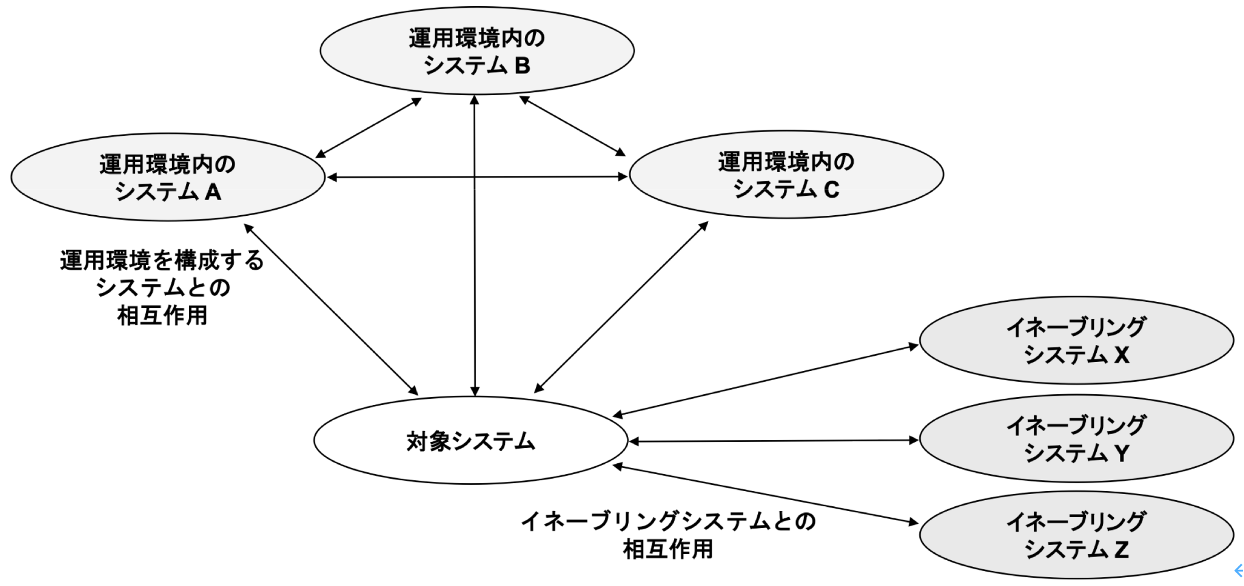
\includegraphics[width=100mm,bb=0 0 622 293]{safety_assurance_contents/ch4images/fig1.png}
    \caption{イネーブリングシステム}
    \label{figure:ch4-1}
    \end{center}
\end{figure}

\subsection{システムの開発や運用においてありうる活動の定義}

システムエンジニアリングでは、システム開発に関わる活動を分類し、標準化
したものとしてシステムライフサイクルプロセス(system lifecycle
  processes)が定義されています。ISO/IEC/IEEE 15288:2023による定義を
図~\ref{figure:ch4-2}に示します。
\begin{figure}
    \begin{center}
    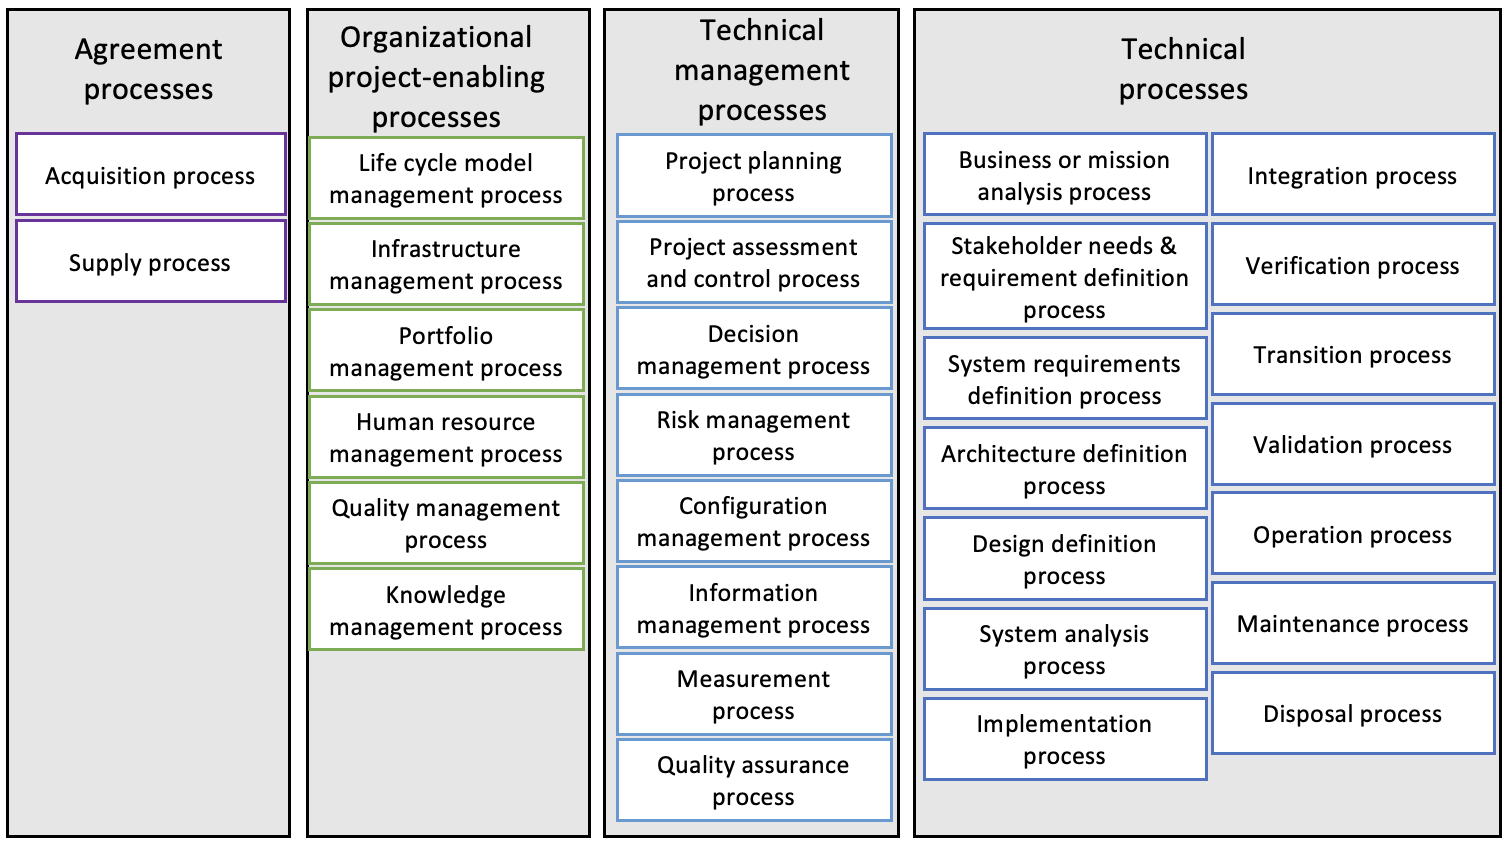
\includegraphics[width=100mm,bb=0 0 756 424]{safety_assurance_contents/ch4images/fig2.png}
    \caption{システムライフサイクルプロセス}
    \label{figure:ch4-2}
    \end{center}
\end{figure}

システムのライフサイクルに現れる活動は、ここに挙げられているどれかのプ
ロセスに相当すると考えることができます。注意点としては、これらのプロセ
スは順序を定義しているものではないということです。プロセスの順序は、ラ
イフサイクルモデル(lifecycle model)として定義され、異なる概念として
理解されます。

これらのライフサイクルプロセスは以下の4つに分類されます:

\begin{itemize}
    \item 合意プロセス(agreement processes)
    \item 組織のプロジェクトイネーブリングプロセス(organizational project-enabling processes)
    \item テクニカルマネジメントプロセス(technical management processes)
    \item テクニカルプロセス群(technical processes)
\end{itemize}

これらのプロセス群は、システムの直接的な開発活動だけでなく、それを支援
する活動も含んでいます。例えば、テクニカルプロセスには、技術者には馴染
み深い設計定義プロセス(design process)や実装プロセス
(implementation)、運用プロセス(operational process)などが含まれて
おり、イメージしやすいと思われます。一方で、システムズエンジニアリング
で提供されるライフサイクルプロセスはそれらだけではありません。プロジェ
クトを計画するプロジェクト計画プロセス(project planning process)や、
人員の確保や配置などの活動を含む人的リソースマネジメントプロセス
(human resource management process)、さらには、契約に係わる活動であ
る取得プロセス(acquisition process)や供給プロセス(supply process)
などまで含まれています。これは、これまでのシステムズエンジニアリングの
知見において、システムを開発する際には、直接的な開発活動だけでなく、そ
れを支える活動も含めて考える必要があることを表しています。

\subsection{システムを記述するために必要な観点の提供}

システムを開発したり、運用したりするためには、対象システムを記述する必
要があります。その記述方法についてもシステムズエンジニアリングは知見を
与えてくれます。

一般に、大規模なシステムは、一つの設計図だけではその全貌を現すことはで
きません。そのため、例えば、詳細な記述の前に、その概要だけを記した文章
や設計図なども作成します。従来からそのような記述を「アーキテクチャ設計」
や概要設計と呼んでいました。ただし、概要を把握するにしても、目的やそれ
を読む関係者に応じて複数の記述を作成することが一般的です。それではどの
ような記述が「アーキテクチャ」とよべるのでしょうか。アーキテクチャの記
述は一般にはシステムの抽象的なものです。ただし、抽象的であればアーキテ
クチャというわけでもありません。なぜ抽象化された記述なのに、それが利用
されるかと言えば、システムに関する何らかの関心事を表していたり、懸念事
項を確認できたりすることが期待されるからです。また、ここでの「関心事」
や「懸念事項」は、それを持つ主体が想定されます。システムに関して関心や
懸念を持つ主体を広くステークホルダー(stakeholder, 利害関係者)と呼び
ます。ここで、なんらかのしステークホルダーのなんらかの関心事(concern)
を表現したものをアーキテクチャビュー(architecture view)と呼びます。
アーキテクチャ記述(architecture description)は、このビューの集まりで
あると定義されます。

さらに、ステークホルダーとその関心事は、典型的なものはパターン化してお
くと便利であり、かつ、その記述方法は、おのずと適切に表現できる記法がき
まってくることが多いです。このような、ステークホルダーとその関心事、そ
の表現方法をまとめたものをアーキテクチャビューポイント(architecture
  viewpoint)と呼ばれます。アーキテクチャビューとアーキテクチャビュー
ポイントのイメージは次のような図で説明されることがありま
す~(\ref{figure:ch4-3})。

\begin{figure}
    \begin{center}
    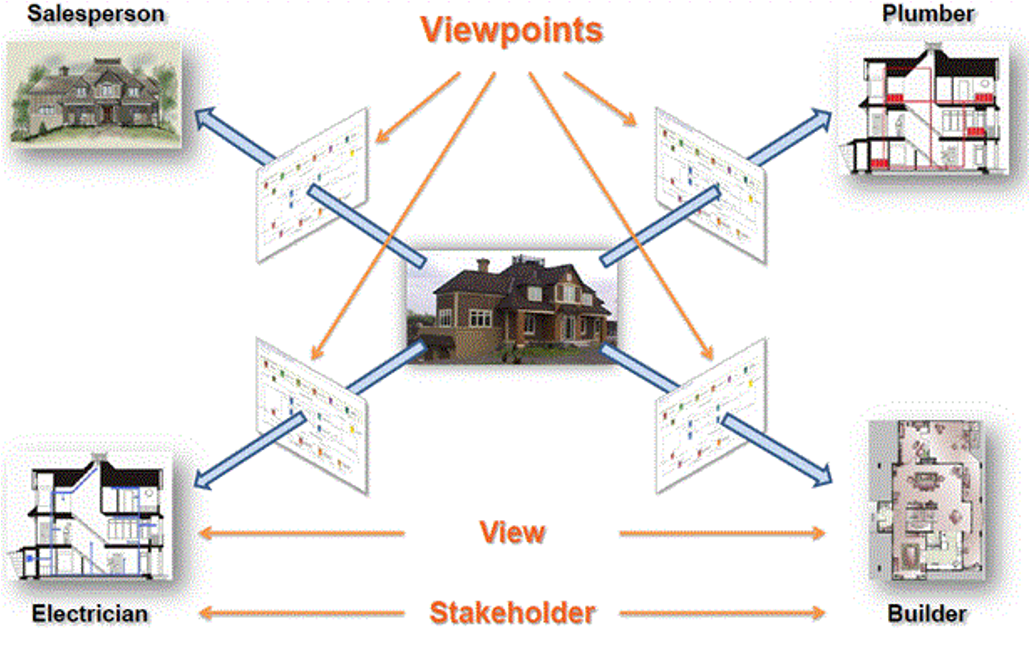
\includegraphics[width=100mm,bb=0 0 515 323]{safety_assurance_contents/ch4images/fig3.png}
    \caption{アーキテクチャビュー及びアーキテクチャビューポイントのイメージ}
    \label{figure:ch4-3}
    \end{center}
\end{figure}

アーキテクチャビューポイントは、原理的にはシステム毎にステークホルダー
やその関心事は異なるため、システム開発のプロジェクト毎に構築しなければ
ならないように見えますが、一般的に多くのプロジェクトで使用可能なアーキ
テクチャビューポイントの集まりもいくつか提供されています。ここでは、そ
れらの情報を用いて、アーキテクチャビューポイントの具体例を紹介します。

\section{モデルベースドシステムズエンジニアリング(MBSE)}

\subsection{MBSEの概念}

モデルベースドシステムズエンジニアリング(model-based systems
  engineering, MBSE)は、モデルを活用したシステムエンジニアリングのア
プローチです。ここでいうモデルとは、ある対象に対して、その対象の特徴を
理解したり予測したりするために用いられる抽象的な表現を指します。

\subsection{SysML(Systems Modeling Language)}

SysMLは、システムエンジニアリングのための代表的なモデリング言語です。
UML(Unified Modeling Language)をベースに定義されており、システムを以
下の四つの側面から記述することが可能です:

\begin{enumerate}
    \item 構造
    \item 振る舞い
    \item パラメータ間の関係
    \item 要求
\end{enumerate}

\section{SysMLを用いたシステムモデリング}

\subsection{構造のモデリング}

構造のモデリングでは、システムを構成する要素とその関係を表現します。例
えば、自動車システムの場合、エンジン、シャーシ、車体などの構成要素とそ
れらの関係を表現します。

\subsection{振る舞いのモデリング}

振る舞いのモデリングでは、システムの動作や状態遷移を表現します。例えば、
自動車の運転プロセスや、エンジンの始動から停止までの状態遷移などを表現
します。

\subsection{パラメータ間の関係のモデリング}

パラメータ間の関係のモデリングでは、システムの性能や特性を決定する要因
間の関係を表現します。例えば、自動車の場合、エンジン出力と最高速度の関
係、車体重量と燃費の関係などを表現します。

\subsection{要求のモデリング}

要求のモデリングでは、システムが満たすべき条件や制約を表現します。例え
ば、自動車の場合、安全性基準、燃費基準、排出ガス規制などの要求を表現し
ます。

\section{トレードオフ分析}

\subsection{トレードオフ分析の概要}

トレードオフ分析は、システムの異なる特性や性能間の関係を評価し、最適な解決策を見出すプロセスです。多くの場合、ある特性を向上させると他の特性が低下するという関係があり、これらのバランスを取ることが重要です。

\subsection{記述型モデルと分析型モデルの連携}

トレードオフ分析を効果的に行うためには、記述型モデルと分析型モデルの連携が重要です。

\begin{itemize}
    \item 記述型モデル:SysMLなどを用いて、システムの構造、振る舞い、要求などを記述します。ステークホルダー間のコミュニケーションや合意形成に役立ちます。
    \item 分析型モデル:MATLAB/Simulinkなどのツールを用いて、システムの性能や動作をシミュレーションします。定量的な評価や予測に役立ちます。
\end{itemize}

\subsection{トレードオフ分析の手順}

以下の手順でトレードオフ分析を行います:

\begin{enumerate}
    \item ソリューション案の検討と妥当性確認
    \item 分析ケースの検討と妥当性確認
    \item パラメータ項目/値の検討と妥当性確認
    \item シミュレーションなどによる分析の実施
    \item 分析結果の評価と意思決定
\end{enumerate}

\section{事例研究: 自動駐車システム}

ここでは、自動駐車システムの設計と評価を例に、システムエンジニアリングの実践を見ていきます。

\subsection{システム概要}

想定する自動駐車システムは以下の特徴を持ちます:

\begin{itemize}
    \item ショッピングセンター近くの巨大な立体駐車場を対象
    \item 利用者は駐車場入口でクルマから降り、アプリで自動駐車を指示
    \item 車両は自律的に空きスペースまで移動し駐車
    \item 引き取り時も、アプリで指示後に車両が自動で出庫
\end{itemize}

\subsection{能力の定義と評価指標}

システムに求められる能力とその評価指標を定義します:

\begin{itemize}
    \item 能力:自動駐車機能
    \item 評価指標:
    \begin{itemize}
        \item 平均入庫時間
        \item 平均出庫時間
        \item 平均待ち時間
        \item 安全度レベル
        \item 利用者ストレスポイント
    \end{itemize}
\end{itemize}

\subsection{リソースアーキテクチャの検討}

システムを構成するリソースとその構造を検討します。主要なコンポーネントには以下が含まれます:

\begin{itemize}
    \item 自動運転機能付き車両
    \item 駐車場管理システム
    \item 空きスペース確認システム(固定カメラまたはドローン)
    \item ユーザーインターフェース(スマートフォンアプリ)
\end{itemize}

\subsection{分析ケースの定義}

システムの評価のための分析ケースを定義します。考慮すべき要素には以下が含まれます:

\begin{itemize}
    \item 自動運転車普及率(例:20%、80%)
    \item 来客状況(閑散期、繁忙期)
    \item 駐車場の構造と容量
    \item 周辺交通状況
\end{itemize}

\subsection{シミュレーションと分析}

定義した分析ケースに基づき、MATLAB/Simulinkなどのツールを用いてシミュレーションを行います。また、STAMP/STPAなどの手法を用いて安全性分析を実施します。

\subsection{結果の評価とトレードオフ分析}

シミュレーションと分析の結果を評価し、各ソリューション案のトレードオフを検討します。例えば:

\begin{itemize}
    \item 固定カメラ方式:初期コストは低いが、スケーラビリティに課題
    \item ドローン方式:柔軟性が高いが、安全管理に追加コストが必要
\end{itemize}

これらの結果を総合的に判断し、最適なソリューションを選択します。

\section{まとめ}

システムエンジニアリングは、複雑なシステムの開発と管理を体系的に行うための重要なアプローチです。MBSEやSysMLの活用、そしてトレードオフ分析の実施により、以下のような利点が得られます:

\begin{itemize}
    \item システムの全体像と詳細の両方を把握できる
    \item ステークホルダー間のコミュニケーションが促進される
    \item 定量的な評価に基づく意思決定が可能になる
    \item システムの品質、信頼性、安全性の向上につながる
\end{itemize}

今後のシステム開発者は、これらの手法と考え方を効果的に活用し、より良いシステムを設計・開発することが求められます。

